\documentclass{article}
\usepackage{graphicx} 
\usepackage{amsmath}
\usepackage{amssymb}
\usepackage[a4paper, total={7in, 9in}]{geometry}

\title{Computer Science Test 2}
\author{Anamaria Sutkova}
\date{January 2025}

\begin{document}

\section*{The Damped Harmonic Oscillator}

The damped harmonic oscillator is a fundamental concept in physics and engineering that describes systems where an oscillatory motion experiences a resistive force proportional to its velocity. Such systems are ubiquitous, appearing in mechanical, electrical, and even biological contexts, such as pendulums, circuits, and molecular vibrations.

\subsection*{Basic Information}
A damped harmonic oscillator consists of three key forces:
\begin{enumerate}
    \item \textbf{Restoring Force}: Provided by a spring or analogous mechanism, proportional to displacement ($-kx$).
    \item \textbf{Damping Force}: Resists motion, proportional to velocity ($-b\dot{x}$), where $b$ is the damping coefficient.
    \item \textbf{External Force}: Optional, often excluded in basic analysis.
\end{enumerate}

The damping force dissipates energy, causing oscillations to diminish over time. The behavior of the system is categorized by the damping coefficient:
\begin{itemize}
    \item \textbf{Underdamped}: Oscillations decay gradually.
    \item \textbf{Critically Damped}: The system returns to equilibrium as quickly as possible without oscillating.
    \item \textbf{Overdamped}: The system returns to equilibrium slowly without oscillating.
\end{itemize}

\subsection*{Equation of Motion}
For a mass $m$, subjected to a restoring force and a damping force, the equation of motion is:
\[
m\ddot{x} + b\dot{x} + kx = 0
\]
where:
\begin{itemize}
    \item $x$ is the displacement,
    \item $\dot{x}$ is the velocity,
    \item $\ddot{x}$ is the acceleration,
    \item $k$ is the spring constant,
    \item $b$ is the damping coefficient.
\end{itemize}

This is a second-order linear differential equation.

\subsection*{Solution for the Equation of Motion}
The solution depends on the damping regime and is found by solving the characteristic equation:
\begin{equation*}
    m\lambda^2 + b\lambda + k = 0
\end{equation*}

The roots $\lambda_1, \lambda_2$ determine the behavior:
\begin{equation*}
    \lambda = \frac{-b \pm \sqrt{b^2 - 4mk}}{2m}
\end{equation*}

\subsubsection*{1. Underdamped Case ($b^2 < 4mk$):}
The roots are complex, leading to a solution of the form:
\begin{equation*}
    x(t) = e^{-\gamma t} \left(A\cos(\omega t) + B\sin(\omega t)\right)
\end{equation*}
where:
\begin{itemize}
    \item $\gamma = \frac{b}{2m}$ (damping factor),
    \item $\omega = \sqrt{\frac{k}{m} - \gamma^2}$ (natural frequency of damped oscillation).
\end{itemize}

\subsubsection*{2. Critically Damped Case ($b^2 = 4mk$):}
The roots are real and equal. The solution is:
\begin{equation*}
    x(t) = (A + Bt)e^{-\gamma t}
\end{equation*}

\subsubsection*{3. Overdamped Case ($b^2 > 4mk$):}
The roots are real and distinct. The solution is:
\begin{equation*}
   x(t) = C_1e^{\lambda_1 t} + C_2e^{\lambda_2 t} 
\end{equation*}

All three possibilities are illustrated in Figure \ref{fig:1}

\begin{figure}[h]
    \centering
    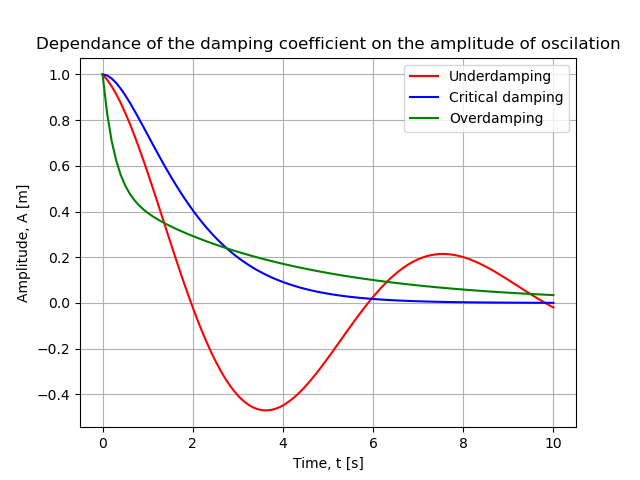
\includegraphics[width=0.8\linewidth]{Fig_test2.png}
    \caption{Graph illustrating three possible damping scenarios}
    \label{fig:1}
\end{figure}

\subsection*{Energy Considerations}
In all cases, the total energy of the system decreases over time due to damping, eventually approaching zero as the system settles into equilibrium.

The damped harmonic oscillator is an essential model for understanding and analyzing dynamic systems where energy dissipation plays a significant role.

\end{document}